\chapter{重修线性代数6——行列式}
	行列式是线性代数中,联系线性方程组解,特征多项式和线性算子标准形式的一个枢纽。在西方科学史上,矩阵起先只是作为行列式所用的表示形式,线性代数的内容早就在这学科形成之前,在行列式的研究中已被了解了。行列式计算的解析表达式,是纯粹用代数方法来讲述这门学问的有力工具,但也因莫名其妙而饱受诟病。
	
	\subsection{行列式的几何含义}
	
	许多教科书都用莱布尼茨公式作为行列式的定义:
	\begin{gather*}
		\begin{vmatrix}a_{11}& a_{12}&\cdots& a_{1n} \\a_{21}& a_{22}&\cdots& a_{2n} \\ \vdots & \vdots&\cdots&\vdots \\a_{n1}& a_{n2} &\cdots& a_{nn}  \end{vmatrix} = \sum_{p}\sigma (p) a_{1p_1}a_{1 p_1}\dots a_{n p_n}
	\end{gather*}

	这里$ p=(p_1,p_2,\cdots, p_n) $ 是数组$  (1, 2,\cdots, n) $ 全排列中的一个置换,共有$ n! $个,$ \sigma(p) $是这置换的奇偶性,奇置换为-1,偶置换是1。这是个纯粹用算法程序来定义的函数,很难看出与经验关联足以想象的含义。这公式定义了行列式作为$ n $阶方阵中$ n^2 $个参数作为变量的多元函数,充满了对称的美、抽象方法的奇妙和构造性计算的确定性。也许教科书的作者想让学生,以此领略抽象代数中一些基本构件的联系,以及代数方法的简洁。但猛然来怎么一下,想看懂它和应用的联系,谁都觉得晕。
	
	在科学理论中列为范本的是欧几里德的几何原理,从简单的几条公理出发,纯粹用逻辑演绎出一套定理,无所不包地解释平面几何中一切关系。现代数学走向公理化的形式逻辑推理,抽象的代数方法无疑是最简洁和严谨的。却没去深思,几何研究面对的是图形,物理概念基于经验,抽象的美好来自于对已知具象的涵盖,驱动推理的灵感是心中的直观想象。除此之外,抽象的概念只是个符合定义条件的约束、什么都可代入的容器,逻辑推理只是句法的机械操作搬弄符号,无关语意,没有灵魂。所以符号主义的人工智能,缺乏人类联想的创作性和驱动推理的方向。高度抽象的数学,是到了高级阶段时对前面知识的总结,只在拥有了丰富的经验内容之后,才能显示出价值。对于初学线性代数的学生,用复杂的算法来定义一个重要的数学概念,会让人迷失在算法的程序中,与现实事物无从接轨。
	
	这里给行列式一个可以想象的几何含义的定义,让你能从图像中“看出”行列式的各种性质。
	
	行列式是用矩阵描写平行多面体广义体积的函数,以正负值来表示行列顺序在空间的定向。
	
	\kaishu
	
	在$ n $维空间中,$ n $个线性无关的向量$ x_1,x_2,\cdots,x_n $构成了一个平行多面体,它的广义体积是以这些向量为变量的多元线性函数$ V(x_1,x_2,\cdots,x_n) $,这函数有下列性质:
	
	1. 单位正交基向量的函数值等于1,$ V(e_1,e_2,\cdots,e_n)= 1 $. ($ n $维单位立方体的体积为1)
	
	2. 	如果变量中有两个向量相等,则函数值为0.(退化平行多面体的体积为0)
	
	3. 	体积函数对其变量具有线性关系,$ V(\cdots, ax+by, \cdots) = aV(\cdots, x, \cdots) + b V(\cdots, y, \cdots) $ 。
	
	\songti
	
	当$ n=2 $时,矩阵描写了平行四边形,$ n=3 $时,它是平行六面体,图形如下,你可以想象高维的情况。$ V $作为广义体积定义的性质,在线性空间的数域是实数时,符合经验的想象。
	
	\begin{figure}[h]
		\centering
		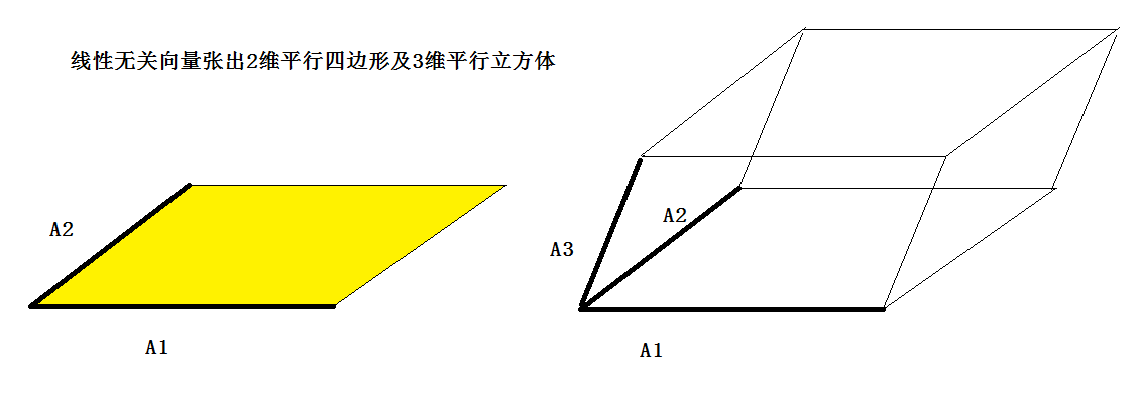
\includegraphics[width=0.7\linewidth]{pic/160908smn6gw0dy66yp37c.png}
		\caption{线性无关向量张出2维评选四边形及3维平行立方体}
		\label{fig:160908smn6gw0dy66yp37c}
	\end{figure}
	
	应用性质2和3,不难推导证明,若变量中两个向量对调位置,则$ V $函数乘上-1,这对应着在高一维的空间中,广义的体积作为与这平行多面体垂直向量的长度时它的朝向。
	
	向量$ x_1,x_2,\cdots,x_n $在标准正交基$ {e_1,e_2,\cdots,e_n} $上,表示为n个列向量$ A_1, A_2,$  $ \cdots,A_n $,用它们组成一个n阶方阵$ A = (A_1, A_2, \cdots,A_n) $,代入不难证明上面的莱布尼茨公式。
	
	列向量也可以直接看成是向量,把它们n个打包成方阵A,A的行列式表示为A到数域的函数,$ |A| = V(A_1, A_2,\cdots,A_n) $,函数值是这些列向量构成的平行多面体的广义体积。
	
	直接从行列式的几何定义出发,很容易想象,任何方阵如果其中的行向量或列向量是线性相关的,它们形成的平行多面体退化成一个低维空间上的几何体,体积为0。所以非零值行列式的矩阵的充要条件是满秩的。
	
	满秩的方阵可以分解为初等矩阵的乘积。任何方阵都可以分解成几个初等矩阵与对角线上只有1和0的对角阵。对角线上有0的对角阵对应着奇异的(不满秩的)方阵,即列向量线性相关,其行列式为零。单位矩阵行列式值为1。在这些初等变换中,数乘变换$ D_i(k) $把其中一个向量变长了k倍,面积也成k倍,列交换Pij改变了向量扫过平行四边形的方向,相反的方向乘上-1,而切变矩阵$ T_{ij}(k) $进行剪切变形,将j轴向i轴方向推斜了k:1斜度,保持体积不变,这些初等变换的行列式值分别等于k,-1,1,所以,方阵的行列式等于分解成的那些初等矩阵与对角阵行列式的乘积。因此,相乘的两个方阵行列式等于它们行列式的乘积。
	
	满秩方阵A的转置等于分解它初等矩阵和对角阵转置后的反向乘积 $ A^{'} $  $= (P_1 P_2\cdots P_k)^{'} = P'_k\cdots P'_2 P'_1 $,而对角阵的转置保持不变,初等矩阵转置后行列式不变,所以转置的矩阵行列式保持不变
	$ \left| A \right| = \left| {A'} \right| $。这意味着上面几何定义的行列式也可以用在行向量,所有对列操作运算的性质对行也适用。
	
	
	
	\subsection{代数余子式与向量的外积}
	
	中学数学里介绍过,三维向量a与b的外积是,它的结果是一个向量$ \textbf a \times \textbf b = \sin \theta \|\textbf a\|\|\textbf b \| \textbf n $,这向量的长度是由a和b形成的平行四边形的面积,方向n是与这平行四边形平面垂直,按右手定则确定的朝向。将这些向量表示成在i, j, k轴的分量形式,可以用行列式的式子来表示:
	
	\begin{gather*}
		\begin{pmatrix}a_1\\a_2\\a_3 \end{pmatrix} \times \begin{pmatrix}b_1\\b_2\\b_3 \end{pmatrix}= \begin{vmatrix}a_1&b_1&i \\a_2& b_2&j\\a_3&b_3&k \end{vmatrix} = \begin{vmatrix}a_1&b_1 \\a_2& b_2 \end{vmatrix}i - \begin{vmatrix}a_1&b_1 \\a_3&b_3 \end{vmatrix}j + \begin{vmatrix}a_2& b_2\\a_3&b_3 \end{vmatrix}k
	\end{gather*}

	这里的i,j,k分别是这些列向量作为坐标表示的单位正交基向量$ e_1,e_2,$  $e_3 $,这个外积向量在这些基向量的分量是这行列式的代数余子式,也可以看成把这两个向量分别投影到与这些基向量垂直的平面上平行四边形的面积。从三维空间中3个向量形成的行列式,可以推出
	
	\begin{gather*}
		\left (  \begin{pmatrix}a_1\\a_2\\a_3 \end{pmatrix} \times \begin{pmatrix}b_1\\b_2\\b_3 \end{pmatrix}\right )\cdot \begin{pmatrix}c_1\\c_2\\c_3 \end{pmatrix} = \begin{vmatrix}a_1&b_1&c_1 \\a_2& b_2&c_2\\a_3&b_3&c_3 \end{vmatrix}
	\end{gather*}

	这里$ \mathbf{a }\times \mathbf{ b} $表示平行四边形面积的法向向量,向量$ \mathbf{c} $对这法向向量的投影与平行四面体面积的乘积$ (\mathbf{a} \times\mathbf{b})\cdot\mathbf{c}$自然是这平行六面体的体积。这个几何的解释完全与行列式的计算一致。
	
	我们感兴趣的是怎么把这个几何直观推到n维空间。把这3个向量放在4维空间,依行列式的计算有
	\begin{gather*}
		\begin{vmatrix}a_1&b_1&c_1 &\textbf e_1\\a_2& b_2&c_2&\textbf e_2\\a_3&b_3&c_3 &\textbf e_3 \\0&0&0 &\textbf e_4\end{vmatrix}  = \begin{vmatrix}a_1&b_1&c_1 \\a_2& b_2&c_2\\a_3&b_3&c_3 \end{vmatrix} \textbf e_4
	\end{gather*}

	这说明行列式计算的广义体积,对应着在高一维空间中与这平行多面体垂直向量的长度。这向量可以用行列式表示为n个向量在n+1维空间上的广义外积。下面进一步解释细节。
	
	教科书都是用公式推导证明,n阶行列式可以按列(行)展开来计算,$ |A| = \sum_{i}a_{ij}D_{ij} $,这里的$ D_{ij} $叫做$ a_{ij} $的代数余子式,它是矩阵$ A $中划去第$ i $行第$ j $列后n-1阶行列式的值乘上$ (-1)^{i+j} $。这低一阶的行列式如法炮制,又可以用再低一阶的行列式来计算,这种递归算法叫做拉普拉斯定理。然而,从几何解释中直接看出这一点,将给我们更清晰的图像理解。
	
	对应着A的第j列向量$ A_j $的代数余子式$  (D_{1j},D_{2j}, \cdots, D_{nj})^T $组成代数余子式向量$ D_j $,行列式$ |A|=A_j\cdot D_j $。从行列式是广义体积的几何图像来看,$ D_j $就是n维$ A $矩阵中,除去$ A_j $余下的n-1个向量,张成n-1维空间里平行多面体的广义体积。这n-1维的广义体积的向量与它所在的子空间垂直,它与$ A_j $的内积作为“面积”与“高”的相乘,构成n阶行列式的广义体积。
	
	代数余子式向量可以看做三维空间中两个向量外积概念的推广,从三维空间中两个向量平行四边形面积为长度的法向向量,推广到n维空间n-1个向量平行多面体广义体积为长度的法向向量。代数余子式$ A_{ij} $是对应于j的法向向量对第i坐标轴的投影,这法向量与多面体所在的子空间垂直,相当于这多面体向与第i坐标轴垂直的子空间的投影,所以在计算广义体积时,不计这n-1个向量在第i坐标轴上的分量,在构造余子式的n-1阶子行列式中,需要移动矩阵A的第j列移和第i行到子行列式外,其中交换列和行$ 2n-i-j $次,所以代数余子式要乘上$ (-1)^{i+j} $因子。
	
	一般形式的拉普拉斯定理,把这种三维空间中“高”与“面积”的相乘得到“体积”的思路,进一步推广到n维空间广义体计算积中,用k阶行列式的子式表示的投影到“高”那k维部分的向量,与n-k阶代数余子式表示的“面积”部分向量的内积。
	
	如果你还没有形成足够的空间想象能力,能通过上面的描述看到几何图像,建议用上面二维和三维空间行列式和向量外积计算,在纸面上画出图形来理解。线性代数课是继平面几何,解析几何之后,对抽象的空间想象能力的训练。抽象概念的想象也是在课程学习中,逐步建立起来能够看到的画面,在学习中忽视了这一点,你就无法看到进一步学习内容中的图像。
	
	\subsection{逆矩阵和克莱姆公式}
	
	矩阵$ A = (\mathbf{A_1},\mathbf{ A_2}, \cdots,\mathbf{A_n}) $的代数余子式向量构成的矩阵$ D = (\mathbf{D_1}, \mathbf{D_2},$  $\cdots,\mathbf{D_n}) $的转置,叫做$ A $的伴随矩阵。代数余子式向量与张成它的n-1阶多面体垂直,$ D_i·A_j = 0,i \neq j $;由拉普拉斯定理有$ D_j\cdot A_j = |A| $,所以$ D^TA = |A|I $,这得出非奇异方阵的逆的解析表达式$  A^{-1} = D^T/|A| $。
	
	对于线性方程组$  Ax = c $,将$ A $的伴随矩阵左乘方程两边,则得到$ |A|x = (D_1, D_2, \cdots,D_n)^Tc $,所以x的第i个分量有$ |A|x_i = D_i\cdot c $,由6.2节中拉普拉斯定理的解释得知这个内积等于行列式$ |D_1, D_2,\cdots D_{i-1},c,D_{i+1},D_n| $,当$ A $是非奇异时则有克莱姆公式$ x_i=|D_1, D_2, \cdots D_{i-1},c,D_{i+1},D_n|/|A| $。
	
	行列式是个有确定结果的算法表达式。无论是求矩阵的逆还是线性方程的解,以及以后的各种应用,都能用它得出解析的式子,这在理论上有很大意义。但是由于它的计算量与其阶数成指数函数关系,所以除了2阶等极端情况外,在实践中都是先将矩阵变换成三角阵或准三角阵后再行计算。
	
	\subsection{张量和半张量积}
	
	行列式的值对于它的列向量(或行向量)都有线性关系,它可以看成是一种斜对称的多线性函数,向量的内积是两个变量的对称双线性函数。研究多线性代数的数学称为张量分析。张量是用来表示在标量、向量和其他张量之间线性关系的多线性函数。它是一种比向量更广泛意义上的“数量”,它的概念可以包括标量、向量、线性算子等等作为特殊情况。在线性空间上线性作用的重数称为张量的“阶(rank)”,标量可以看作是0阶的张量,向量是1阶的,线性算子是2阶的。在给定的坐标下,向量表示为1维的数组(即列向量),线性算子为2维的数组(即矩阵),r阶张量为r维数组。在坐标变换中依变换的方式不同,其指标可以分成协变和逆变两种,具有丰富的表达能力,在物理和工程上有着广泛的应用。
	
	高维数组在数学和工程问题上经常使用,尤其应用在对多线性和非线性问题的处理,但在显示和分析上十分不便。如果把它们按一定的顺序排成一列或矩阵,规定它们间合适的运算规则,则既可以方便地在书面上显示、作理论分析,又能与原来的数组运算等价。这种新的矩阵运算叫做“半张量积”,是对普通矩阵乘法进行推广。传统上矩阵的乘法AB,要求A的列数与B的行数相等,相乘时A 与B中的相应的元素是1对1的运算;矩阵的张量积没有这限制,它是A中的每个元素与整个B矩阵来相乘,但它与传统矩阵乘法不能兼容;而半张量积与张量积一样,对A、B矩阵的列行数并无要求,其运算规则介乎传统乘法与张量积之间,当列行数相等时即为传统的矩阵乘法,但有倍数关系时就变成其中一个矩阵元素与另一矩阵按倍因子分块配对的乘法,进而推广到任意的两个矩阵。半张量积的这种矩阵运算规则,不仅适用于多维数组排成矩阵后的等价运算,而且它与矩阵的加法有分配律,与矩阵通常乘法有结合律,这是一种漂亮地解决多维数组书面表达、分析、计算和扩展矩阵乘法的设计。这是程代展教授对矩阵理论的原创性贡献,经过十多年普及,现已成为表达有限集合上映射及性质,研究有限集合上的动态系统的演化规律及控制的有力工具,在动力系统、网络、线路设计与检测等方面有许多应用。\\
%\\[12pt]
	
	【补充】贴在评论[10]之后
	
	一些读者对半张量积好奇,希望给个简单的例子。这里简介一下。
	
	定义:设A是$ m\times n $矩阵,B是$ p\times q $矩阵,记$ n $与$ p $的最小公倍数为$ t  $. 定义$ A $与$ B $的半张量积为
	\begin{gather*}
		  (A\bigotimes It/n)(B\bigotimes It/p) 
	\end{gather*}
	这里$ \bigotimes $是矩阵的张量积(Kroneckerproduct)。
	
	注:上述定义中,如果n=p称A与B是等维数,如果n与p其中一个能整除另一个,则称是倍维数的, 其他为一般情况。定义是对一般情况给出的。对于等维数的情况, 它退化为普通矩阵乘法,倍维数可简化为分块积。因此, 半张量积是普通乘法的推广。倍维数情况定义左半张量积是最常用的。在这定义下结合律与分配律对半张量积仍成立。
	
	仍然觉得晕?好吧,举例说明。张量积$ A\bigotimes B $意思是A中每一个元素与每一个B中元素相乘的矩阵,或者说A中每一个元素与整个B相乘,然后按A的布置排出的矩阵,比如说:
	\begin{gather*}
		B=\begin{pmatrix}1 &2 \\-1&3\end{pmatrix},I_2=\begin{pmatrix}1 &0\\0&1\end{pmatrix},B\bigotimes I_2=\begin{pmatrix}1 & 0 &  2& 0\\ 0 & 1 &  0& 2\\  -1&  0&  3& 0\\ 0 & -1 &  0& 3\end{pmatrix}
	\end{gather*}

	假如A是3x4的矩阵,B如上是2x2的矩阵,它们的最小公倍数是4,I1是1,A与B的半张量积 $ A\circledast B $ 如下(注:$ \circledast $ 不是半张量积的标准符号,只是无法找到这标准符号,暂时用它聊以示意)
	\begin{gather*}
		A=\begin{pmatrix}1 & 2 & -1& 2\\ 0 & 1 &  2& 3\\  3&  3&  1& 1\end{pmatrix}, A\circledast  B = A(B\bigotimes I_2)=\begin{pmatrix}2 & 0 & -1& 10\\ -2 & -2 & 6& 11\\2& 2& 9& 9\end{pmatrix}
	\end{gather*}
	
	因为这是倍维数的半张量积,也可以把它化简为A中的列分成2块与B向乘。
	\begin{gather*}
		A_1=\begin{pmatrix}1 & 2 \\ 0 & 1 \\  3&  3\end{pmatrix}, A_2=\begin{pmatrix} -1& 2\\ 2& 3\\ 1& 1\end{pmatrix},\\
		A\circledast B =\begin{pmatrix}A_1 & A_2\end{pmatrix}\begin{pmatrix}1 &2 \\-1&3\end{pmatrix}=\begin{pmatrix}A_1-A_2 & 2A_1+3A_2\end{pmatrix}=\begin{pmatrix}2 & 0 & -1& 10\\ -2 & -2 & 6& 11\\2& 2& 9& 9\end{pmatrix}		
	\end{gather*}

	为什么定义这样的乘法?想一想A原来是个3x2x2的三维数组展成的矩阵,A1,A2是三维数组的第三个下标的两个断面,为了显示方便把它们并排放一起变成一个矩阵,这第三个下标方向按传统方式与B来相乘(想象一下线性算子的复合),然后再把它们排放成一个矩阵。想进一步了解它的理论和应用,详见:
	
	1. 程代展, 赵寅. 矩阵的半张量积: 一个便捷的新工具. 科学通报, 2011, 56: 2664–2674
	
	2. 程代展,齐洪胜,矩阵的半张量积理论与应用,科学出版社,2007